\documentclass[12pt, oneside]{article}   	% use "amsart" instead of "article" for AMSLaTeX format
%\documentclass[12pt, oneside, draft]{article}   	% use "amsart" instead of "article" for AMSLaTeX format

%%%%%%%%%%%%%%%%%%%%%%%%%%%%%%%%%%%%%%%%%%%%%%%%%
%
% The TexLive distribution is stored in /usr/local/texlive/2020
%
% The definitions of the packages are in /usr/local/texlive/2020/texmf-dist/tex/latex
%
%%%%%%%%%%%%%%%%%%%%%%%%%%%%%%%%%%%%%%%%%%%%%%%%%

\usepackage{xparse}					% Allows for the creation of \NewDocumentCommand shortcuts

\usepackage{geometry}				% See geometry.pdf to learn the layout options. There are lots.
\geometry{letterpaper}				% ... or a4paper or a5paper or ... 
\usepackage[parfill]{parskip}		% Activate to begin paragraphs with an empty line rather than indent
\usepackage{float}					% Float package to exert more control over graphic placement
	
%\usepackage{verbatim}				% Creates a verbatim environment for code / program output
\usepackage{graphicx}				% Use pdf, png, jpg, or eps§ with pdflatex; use eps in DVI mode
									% TeX will automatically convert eps --> pdf in pdflatex
\graphicspath{{./figures/}}         

% Math packages
\usepackage{amssymb}				% Mathematical symbols
\usepackage{amsmath}				% Added for typesetting mathematical formulae
\usepackage{amsthm}					% Added for typesetting mathematical theorems
\usepackage{mathalpha}				% Added for some special characters like Q, Z and N

% Table packages in addition to built in tabular
\usepackage{booktabs}				% Adds extra commands to tabular like \toprule
\usepackage{afterpage}				% For pagination support
\usepackage{longtable}				% Support for longer tables

% Hyperlinks
\usepackage{hyperref}				% For creating internal and HTTP links

% Numbering and references
\numberwithin{equation}{section}          % Number equations within sections
\usepackage[numbers]{natbib}              % For bibliography management

% For Tikz graphics
\usepackage{tikz}					% Package for pgf and TikZ
\usetikzlibrary{shapes,arrows,chains}
\tikzstyle{startstop} = [very thick, rectangle, rounded corners, minimum width=2.5cm, minimum height=0.8cm, text centered, draw=black, text width=2.5cm]
\tikzstyle{action} = [rectangle, rounded corners, minimum width=3cm, minimum height=0.8cm, text centered, draw=black, text width=2.5cm]
\tikzstyle{decision} = [diamond, minimum width=3cm, minimum height=3cm, text centered, draw=black, text width=2cm]
\tikzstyle{arrow} = [thick,->,>=stealth]

% For theorems and definitions - each creates it's own counter which incrementa each use
\theoremstyle{definition}
\newtheorem{proposition}{Proposition}[section]
\newtheorem{define}{Definition}[section]
\newtheorem{axiom}{Axiom}[section]
\newtheorem{theorem}{Theorem}
\newtheorem{lemma}[theorem]{Lemma}
\newtheorem{corollary}[theorem]{Corollary}
\newtheorem*{remark}{Remark}

%SetFonts


\title{On the Asymptotic Density of Convergent Residue Classes in the Collatz Map}
\author{Wayne Brassem}
%\date{}							% Activate to display a given date or no date


\begin{document}

% Document define commands for commonly used items in math mode
\NewDocumentCommand{\setN}{}{\mathbb{N}}				% Set of positive integers, excluding 0
\NewDocumentCommand{\setNo}{}{\mathbb{N}_0}				% Set of positive integers, including 0
\NewDocumentCommand{\setNeven}{}{\mathbb{N}_{even}}		% Set of even positive integers, excluding 0
\NewDocumentCommand{\setNodd}{}{\mathbb{N}_{odd}}		% Set of odd positive integers
\NewDocumentCommand{\setZ}{}{\mathbb{Z}}				% Set of all integers, excluding zero
\NewDocumentCommand{\setZo}{}{\mathbb{Z}_0}				% Set of all integers, including zero
\NewDocumentCommand{\setQ}{}{\mathbb{Q}}				% Set of all rational numbers

% Document define commands for commonly used items not in math mode
\NewDocumentCommand{\Rarr}{}{\textrightarrow{}}			% Right arrow

% Document commands which provide hyperlinks to OEIS sequences referenced herein
\NewDocumentCommand{\OEIS}{m}{\href{https://oeis.org/#1}{#1}}

\maketitle



\begin{abstract}

We investigate the iterative dynamics of the classical Collatz map
\[
g(x) = \begin{cases}
\displaystyle
    \phantom{3x} \frac{x}{2} & \text {if } x \text{ is even}, \\[4pt]
\displaystyle
    3x+1        & \text {if } x \text{ is odd},
\end{cases}
\]
on the positive integers by encoding trajectories as finite sequences of
parity-determined steps. Each such sequence — a \emph{parity word} describing
the pattern of odd and even steps along an orbit — uniquely determines a
residue class modulo a power of two. These residue classes are disjoint, and
those corresponding to \emph{convergent} parity words consist of integers that
reach a strictly smaller value under finite iteration.

By developing a complete combinatorial characterization of admissible parity
words and their associated division counts, we assign a well-defined asymptotic
density to each convergent residue class. Organizing these classes by minimal
stopping time yields finite disjoint families whose cumulative densities increase
monotonically.

We show that the density contribution of newly appearing convergent residue
classes vanishes as the stopping time grows, and consequently that the total
asymptotic density of convergent residue classes approaches one. Thus,
convergent behavior dominates the Collatz map in the sense of natural density.
Any exceptional trajectories, should they exist, must therefore be confined to
a set of density zero.

\end{abstract}


\tableofcontents
\newpage


\section{Introduction}

\subsection{The Collatz Mapping and Known Results}

The Collatz conjecture concerns the iteration of a simple piecewise-defined map
introduced by Lothar Collatz in 1937~\cite{Collatz1937}, defined as follows.

\begin{define}[Standard Collatz Map]
\label{def:standard-map}
The \emph{standard Collatz map} $g : \setN \to \setN$ is defined by
\[
g(x) =
\begin{cases}
\displaystyle
    \phantom{3x} \frac{x}{2} & \text {if } x \text{ is even}, \\[8pt]
\displaystyle
    3x+1,                    & \text{if $x$ is odd}.
\end{cases}
\]
\end{define}

In this paper, we primarily study the accelerated map defined below on the
positive integers.  All results are stated in terms of the accelerated map
\( f \), which is dynamically equivalent to the standard Collatz map \( g \)
in the sense that each orbit of \( g \) corresponds to an orbit of  \( f \)
obtained by collapsing consecutive divisions by two, and vice versa. 

\begin{define}[Accelerated Collatz Map]
\label{def:accelerated-map}
The \emph{accelerated Collatz map} is the function
\( f : \setN \rightarrow \setN \) defined by
\[
f(x) = \begin{cases}
\displaystyle
    \phantom{3x} \frac{x}{2} & \text {if } x \text{ is even}, \\[8pt]
\displaystyle
    \frac{3x+1}{2}           & \text {if } x \text{ is odd}. \\
\end{cases}
\]
This map acts on the positive integers and combines each odd step of the classical Collatz
iteration \(x \mapsto 3x+1\) with the immediately following division by two
\cite{Everett1977}.
\end{define}

The Collatz conjecture asserts that, under iteration of $f$, every positive
integer eventually reaches the trivial cycle $2 \to 1 \to 2$, which corresponds
to the classical $4 \to 2 \to 1 \to 4$ cycle under the standard map $g$
\cite{Collatz1937}.

Despite its elementary formulation, the conjecture has resisted proof for decades
\cite{Lagarias2010,Terras1976}. Extensive computational verification confirms convergence
for all integers up to very large bounds \cite{OliveiraESilva2010}, but such verification
does not constitute a proof and offers limited insight into the global structure
of Collatz trajectories.

In addition to trajectory-by-trajectory analysis and probabilistic heuristics
\cite{Wirsching1998}, a substantial body of work has examined the problem from a more
structural and arithmetic perspective, including the use of residue classes, stopping
times, affine representations, and combinatorial encodings of parity patterns
\cite{Terras1976,Everett1977,Lagarias2010}. These approaches reveal important regularities
in the dynamics but have not, to date, yielded a mechanism that controls the behavior
of all trajectories simultaneously across the positive integers.


\subsection{Strategy of the Proof}

This paper adopts a structural approach based on decomposing the positive integers into
arithmetic residue classes determined by parity patterns under the accelerated Collatz map.

The central idea is to study finite Collatz paths abstractly and to associate each such path
with a residue class of integers that follow the same parity pattern for a fixed number of
odd steps. These classes are pairwise disjoint and together form a partition of the positive
integers. Each class is assigned a minimal stopping time, defined as the first iterate at
which all elements of the class map to a value strictly smaller than their initial value.
The key novelty is to control the global \emph{density behavior} of these classes by
analyzing the grammar of admissible parity words and the multiplicative growth they permit.

The analysis proceeds through the following steps:

\begin{itemize}
\item Encode Collatz trajectories using parity words that record the number of divisions by
      two between successive odd steps.
\item Show that each admissible parity word (i.e., one satisfying the prefix-wise growth
      constraint) determines either an empty set or a single arithmetic residue class of
      positive integers, and that these classes are pairwise disjoint.
\item Prove that convergent residue classes of fixed stopping time are pairwise disjoint.
\item Express the asymptotic density of each such class in terms of its total division count.
\item Analyze the grammar of admissible parity words to classify the possible local growth
      patterns and to establish rigorous upper bounds on the multiplicative growth associated
      with each pattern.
\item Show that the locally maximal growth pattern corresponds to a $5$--cycle whose infinite
      repetition violates admissibility under the prefix-wise constraint. This formally
      inadmissible extremal word provides a strict upper envelope for the growth of all
      admissible parity words.
\item Deduce that the density contribution of newly appearing convergent classes tends to
      zero as the stopping time increases, so that the union of all convergent residue
      classes has asymptotic density one.
\end{itemize}

Thus, within the explicit partition of the positive integers induced by parity patterns,
almost every integer (in the sense of asymptotic density) belongs to a residue class whose
elements decrease after finitely many iterations. The analysis does not exclude the
possibility of exceptional trajectories lying outside these convergent classes, but shows
that any such set must have asymptotic density zero.


\section{Definitions and Preliminaries}

\subsection{Stopping Time}

\begin{define}
The \emph{stopping time} \( \sigma(x) \) of a positive integer \(x\) (sometimes called the finite
stopping time or local descent time) is the minimal integer
\(k \in \setN\) (if such a \(k\) exists) such that
\[
f^k(x) < x.
\]
If no such \(k\) exists, we write \(\sigma(x) = \infty\). Stopping time behavior has been studied
extensively in the context of the $3x+1$ problem \cite{Terras1976}.
\end{define}


\subsection{Convergent Segments}

\begin{define}
A \emph{convergent segment of length \(k\)} is a finite sequence
\[
x, f(x), f^2(x), \ldots, f^k(x)
\]
such that \( f^k(x) < x \) and \(k\) is minimal. No assumption is made about eventual
convergence to 1; only strict descent at step \(k\), i.e., \(k = \sigma(x)\), is required.
Finite segments of this type were considered in the context of the accelerated Collatz map
by Everett \cite{Everett1977}.
\end{define}


\subsection{Residue Classes}

\begin{define}
Two positive integers \(x,y \in \setN\) are said to be in the same \emph{residue class of
depth \(k\)} if their first \(k\) Collatz iterates are identical. Encoding trajectories
via residue classes or arithmetic progressions has appeared in prior structural approaches
to the $3x+1$ problem \cite{Wirsching1998,Chamberland2003}.
\end{define}

\medskip
\noindent\textit{Indexing convention.}
Iterates are indexed starting from \(0\), so that \(f^0(x)=x\) and agreement of the first
\(k\) iterates means equality for indices \(i=0,\dots,k-1\). This convention aligns with
the 0-based combinatorial and OEIS sequences used in the analysis.

\begin{define}[Residue Class of Depth \(k\)]
\label{def:residue-class}
Fix \(k \in \setN\) and \(x \in \setN\). The \emph{residue class of depth \(k\) with
respect to \(f\)} containing \(x\) is
\[
[x]_k := \{ y \in \setN \mid f^i(y) = f^i(x) \text{ for } i = 0, 1, \dots, k-1 \}.
\]
\end{define}

\begin{define}[Convergent Residue Class]
A residue class \([x]_k\) is called \emph{convergent of stopping time \(k\)} if:
\begin{enumerate}
\item \( f^k(y) < y \) for all \( y \in [x]_k \), and
\item for every \( y \in [x]_k \), no smaller integer \( j < k \) satisfies \( f^j(y) < y \).
\end{enumerate}
Here \(k\) is minimal with this property across the entire class.
\end{define}

\begin{remark}
This definition is stronger than requiring \(\sigma(x)=k\) for a single representative
\(x\), since it enforces uniform descent at step \(k\) for all elements of the residue class.
\end{remark}


\section{Division Counts and Path Encoding}
\label{sec:division-counts}

The structure of convergent residue classes is governed by the total number
of divisions by two incurred along a Collatz path. This number depends only
on the \emph{parity pattern} of the path, understood as the sequence of
divisions by two following each odd step, and not on the specific starting
integer.

In this section we introduce a symbolic encoding of Collatz trajectories
based on the number of divisions by two occurring after each odd step.
We call such an encoding a \emph{parity word}. The precise combinatorial
constraints determining which parity words correspond to actual trajectories
are deferred to Section~\ref{sec:grammar}; however, the definitions
given here are sufficient for the analysis of residue class densities.


\subsection{Formal Definition of Parity Words}

\begin{define}[Parity Word]
A \emph{parity word} of length \(k \ge 0\) is a finite sequence
\[
\omega = (d_0, d_1, \dots, d_{k-1}),
\]
where each \(d_i \in \setN_{\ge 0}\) records a symbolic count of divisions by two
associated with the $i$-th odd step of an accelerated Collatz iteration
(indexing starts at $i=0$). 

For \(k=0\), the sequence is empty and corresponds to a trajectory with no
odd steps.
\end{define}

Each parity word formally determines a linear-affine transformation
\begin{equation}
\label{eq:linear-affine-map}
x \longmapsto \frac{3^k x + c(\omega)}{2^{d_0+\cdots+d_{k-1}}},
\end{equation}
obtained by symbolic composition of the accelerated Collatz map along the word.
Here \(c(\omega)\) is a canonical integer uniquely determined by the parity word
(see Appendix~\ref{app:canonical-c}). This representation encodes the arithmetic
effect of the sequence of odd and even steps on any starting integer.

\begin{remark}[Parity Words Encode Structure, Not Values]
Fixing a parity word $\omega$ determines the sequence of arithmetic
operations applied along an accelerated Collatz trajectory. Consequently,
both the linear coefficient \(3^k/2^{d_0+\cdots+d_{k-1}}\) and the affine term
\(c(\omega)\) depend only on $\omega$ and not on the starting integer.

This allows us to reason about convergence or divergence at the level of
residue classes without reference to specific integers.
\end{remark}

\begin{remark}[Residue Classes and Parity Words]
Every parity word $\omega$ determines a unique residue class $[x]_k$ of depth $k$ under $f$, 
consisting of all integers whose first $k$ iterates under $f$ follow the divisions encoded by $\omega$.
\end{remark}


\subsection{Total Division Count}

Let a Collatz path contain exactly $k$ odd steps (``up-legs''). Between
successive odd steps, the accelerated Collatz map applies a finite number
of divisions by two. The cumulative number of such divisions determines
the arithmetic structure of the corresponding residue class.

\begin{define}[Total Division Count]
Let $k \ge 0$. For a given parity word $\omega = (d_0,\dots,d_{k-1})$,
define its \emph{total division count} by
\[
D(\omega) := \sum_{i=0}^{k-1} d_i.
\]
\end{define}

The integer $D(\omega)$ is precisely the exponent of $2$ appearing in the
denominator of the linear-affine form of the $k$-step iterate (see
Equation~\eqref{eq:linear-affine-map}).  

\begin{remark}[Empty Parity Words and Purely Even Trajectories]
The case $k=0$ corresponds to \emph{empty parity words}, representing trajectories
with no odd steps before descending below their starting value. These are
precisely the powers of two, which satisfy $f^m(x)=x/2^m$ for all $m$ and hence
are trivially convergent. While $k=0$ does not define a nontrivial residue class,
it serves as a degenerate base case and requires no separate treatment in the
density analysis.
\end{remark}

Parity words with the same number of odd steps may differ in the
distribution of divisions by two between steps and hence in their total
division count. However, for each parity word, its total division count
$D(\omega)$ is uniquely determined by the sequence of divisions encoded
in the word.

\begin{define}[Minimal Total Division Count]
Let $A020914(k)$ denote the minimal total number of divisions by two among
all \emph{admissible} parity words containing exactly $k$ odd steps.
\end{define}

This quantity is given by $\lceil \log_2(3^k) \rceil$, a fact derived in
Section~\ref{sec:grammar} and tabulated in \OEIS{A020914}. Intuitively,
each odd step multiplies the trajectory by $3$, so the cumulative divisions
by two must at least balance this growth; hence the minimal total division
count corresponds to the smallest exponent of $2$ that offsets the factor
of $3^k$ in the linear-affine map for a path with $k$ odd steps.


\subsection{Density of Residue Classes}

\begin{lemma}[Disjointness of Residue Classes]
For fixed $k$, the residue classes induced by distinct parity words are pairwise disjoint.
\end{lemma}

\begin{proof}
Each parity word with $k$ odd steps and total division count $D$
determines a unique residue class of the form
\[
n \equiv r \pmod{2^{D}},
\]
with exactly one representative per period of length $2^{D}$. Indeed, the
associated linear-affine form
\[
x \longmapsto \frac{3^k x + c(\omega)}{2^{D}}
\]
has denominator $2^{D}$, and integrality of the iterate forces $x$ to lie in a
unique congruence class modulo $2^{D}$.

If two distinct parity words produced the same residue class, then the same
integrality constraints would apply, forcing identical parity decisions at
each step. This would imply that the two words encode the same sequence of
operations, contradicting their distinctness. Therefore, distinct words
correspond to distinct residue classes, and the associated classes are
disjoint.
\end{proof}

\begin{proposition}
A residue class with total division count $D$ has asymptotic (natural) density
\[
2^{-D}.
\]
In particular, for any class with $k$ odd steps,
\[
\text{density} \le 2^{-A020914(k)}.
\]
\end{proposition}

\begin{proof}
Each class is an arithmetic progression with step size $2^{D}$
and exactly one representative per period. The result follows immediately.
\end{proof}

\begin{remark}
At fixed $k$, there are finitely many distinct convergent residue classes, since
only finitely many parity words of length $k$ exist. Let $\widetilde A(k)$ denote
the number of such classes. Since these classes are pairwise disjoint, their
total density contribution at stopping time $k$ is
\[
\widetilde A(k)\,2^{-A020914(k)}.
\]
\end{remark}

\subsection{Example}

For convergent segments with $k=4$ odd steps, the minimal total division
count is $A020914(4)=7$. For parity words attaining this minimum, the
associated residue classes consist of integers of the form
\[
x = 2^7 n + r, \quad n \in \setN,
\]
where the residue $r$ depends on the specific parity word. Each residue $r$
modulo $2^7$ corresponds uniquely to a parity word of length $4$ achieving
the minimal division count, so the residue class $[x]_4$ is fully determined
by the parity structure of the trajectory.

This example illustrates that convergent behavior depends only on parity
structure and accumulated division count, motivating an abstract
description of Collatz trajectories independent of their starting values.


\section{Grammar of Collatz Parity Words}
\label{sec:grammar}

\subsection{Parity Words as Dynamical Encodings}

\begin{remark}[Parity Grammar as a Dynamical Encoding]
Recall from Section~\ref{sec:division-counts} that a \emph{parity word}
$\omega=(d_0,\dots,d_{k-1})$ records the number of divisions by two applied
after each odd step of an accelerated Collatz trajectory.

The parity-word grammar introduced in this section provides a symbolic
encoding of accelerated Collatz dynamics, following the symbolic approach
of Chamberland~\cite{Chamberland2003}. This encoding is not injective:
multiple positive integers can correspond to the same parity word.
Specifically, distinct integers whose trajectories share the same sequence
of division counts after $k$ odd steps map to the same parity word, forming
the arithmetic residue classes described in
Section~\ref{sec:division-counts}.

Unlike a purely combinatorial encoding, parity words retain essential
dynamical information. Each parity word $\omega=(d_0,\dots,d_{k-1})$
determines the sequence of multiplicative factors
\[
r_i = \frac{3}{2^{d_i}},
\]
so that the contractive or expansive contribution of each odd step is
preserved at the level of the linear coefficient (with the affine term
handled separately via $c(\omega)$). This structure will allow us to
quantify densities of residue classes and to formulate sufficient
conditions for descent, even though individual trajectories are collapsed
under the encoding.
\end{remark}

\subsection{Admissibility of Parity Words}

\begin{define}[Admissible Parity Word]
\label{def:admissible-parity-word}
Let $\omega = (d_0, \dots, d_{k-1})$ be a parity word and write
$D = d_0+\cdots+d_{k-1}$. Associated to $\omega$ is the affine map
\[
T_\omega(x) = \frac{3^k x + c(\omega)}{2^{D}},
\]
where $c(\omega)$ is the canonical integer determined by $\omega$.

The parity word $\omega$ is said to be \emph{admissible} if there exists at
least one integer $x$ such that $T_\omega(x)$ is an integer. Equivalently,
$\omega$ is admissible if the numerator $3^k x + c(\omega)$ is divisible by
$2^{D}$ for at least one residue class of $x \bmod 2^{D}$.
\end{define}

\begin{remark}
Admissibility is therefore an arithmetic condition on the word $\omega$
itself, expressed as a divisibility constraint on the associated affine
map. When this condition holds, the set of all integers $x$ for which
$T_\omega(x)$ is integral forms a single arithmetic progression modulo
$2^{D}$, corresponding to the residue class induced by $\omega$.
\end{remark}

\begin{lemma}[Minimal Division Count]
For any admissible parity word $\omega=(d_0,\dots,d_{k-1})$ of length $k$,
\[
d_0 + \cdots + d_{k-1} \;\ge\; A020914(k),
\]
where $A020914(k)$ denotes the minimal total number of divisions by two among
all admissible parity words of length $k$. This quantity is given by
\[
A020914(k) = \lceil \log_2(3^k) \rceil.
\]

Moreover, equality holds if and only if $\omega$ is admissible with minimal
total division count.
\end{lemma}

\begin{define}[Convergent Parity Word]
An admissible parity word $\omega = (d_0,\dots,d_{k-1})$ is said to be
\emph{convergent} if
\[
\frac{3^k}{2^{d_0+\cdots+d_{k-1}}} < 1.
\]
\end{define}

\begin{remark}[Role of the Affine Term]
The constant term $c(\omega)$ in the affine representation
\[
T_\omega(x) = \frac{3^k x + c(\omega)}{2^{d_0+\cdots+d_{k-1}}}
\]
encodes the cumulative effect of the additive “$+1$” operations arising from
the classical $3x+1$ map along the trajectory determined by $\omega$.
Admissibility ensures that this affine map corresponds to genuine Collatz
dynamics, mapping a nonempty arithmetic progression of integers to integers.
Once admissibility is established, the condition
\[
\frac{3^k}{2^{d_0+\cdots+d_{k-1}}} < 1
\]
characterizes the asymptotic behavior of the map: the associated linear factor
is \emph{contractive}, so that $T_\omega(x) < x$ for all sufficiently large integers
in the corresponding residue class. Thus, although the additive term affects the
finite-scale behavior of individual trajectories, the criterion for convergence
depends only on the multiplicative component of the affine map.
\end{remark}


\subsection{Residue Classes Induced by Parity Words}

Fix a parity word $\omega = (d_0,\dots,d_{k-1})$ of length $k$ that is
admissible in the sense of Definition~\ref{def:admissible-parity-word}.
Let
\[
D(\omega) := d_0 + \cdots + d_{k-1}
\]
denote its total division count. By admissibility,
$D(\omega) \ge A020914(k)$.

\begin{lemma}[Residue Class Modulus]
\label{lem:residue-modulus}
Let $x,y \in \setN$ both realize the same parity word $\omega$, i.e.,
their trajectories under $f$ exhibit the division counts encoded by $\omega$
for the first $k$ odd steps. Then
\[
x \equiv y \pmod{2^{D(\omega)}}.
\]
\end{lemma}

\begin{proof}
For any integer $z$ realizing $\omega$, the $k$ odd steps encoded by $\omega$
induce the affine relation
\[
T_\omega(z) = \frac{3^k z + c(\omega)}{2^{D(\omega)}},
\]
where $T_\omega(z)\in\setN$ by admissibility.
Thus $3^k z + c(\omega)$ is divisible by $2^{D(\omega)}$.

If both $x$ and $y$ realize $\omega$, then
\[
3^k x + c(\omega) \equiv 0 \equiv 3^k y + c(\omega) \pmod{2^{D(\omega)}},
\]
which implies
\[
3^k(x-y) \equiv 0 \pmod{2^{D(\omega)}}.
\]
Since $3^k$ is invertible modulo $2^{D(\omega)}$, it follows that
\[
x \equiv y \pmod{2^{D(\omega)}}.
\]
\end{proof}

\begin{lemma}[Associated Affine Collatz Map]
\label{lem:associated-map}
Each admissible parity word $\omega$ induces a unique affine map
\[
T_\omega(x) = \frac{3^k x + c(\omega)}{2^{D(\omega)}},
\]
where $c(\omega)$ is uniquely determined modulo $2^{D(\omega)}$ by the
requirement that $T_\omega(x)\in\setN$ for all integers $x$ in the residue class
induced by $\omega$.
\end{lemma}

\begin{remark}[Affine Compression of Trajectories]
For any integer realizing a parity word $\omega$, the value $T_\omega(x)$
coincides exactly with the result of applying the accelerated Collatz map
through the $k$ odd steps encoded by $\omega$, including all intermediate
divisions by two. Thus $T_\omega$ represents a compression of a finite
Collatz trajectory into a single affine step.
\end{remark}

\begin{lemma}[Convergent Residue Class]
\label{lem:residue-class}
Each convergent parity word $\omega$ induces a unique arithmetic residue class
\[
x \equiv r_\omega \pmod{2^{D(\omega)}},
\]
whose elements all follow the same parity pattern for $k$ odd steps and satisfy
\[
T_\omega(x) < x.
\]
Consequently, every element of the class reaches a strictly smaller integer
after completing the $k$ odd steps encoded by $\omega$.
\end{lemma}


\section{Increment Grammar and Horizontal-Sum Construction}
\label{sec:increment-grammar}

\begin{remark}[Increment Grammar from Minimal Denominator Growth]
The first difference sequence of $A020914$, given by \OEIS{A022921},
induces a binary \emph{increment grammar} $\{s,d\}$ that describes the growth
of the \emph{minimal admissible} total division count as the number of odd steps increases.

Each symbol records whether the minimal total division count increases by one ($s$) or
two ($d$) when passing from $k$ to $k+1$ odd steps. Importantly, this grammar \emph{does not}
encode the realized parity word entries $d_i$ (which may be arbitrarily large), but rather
governs the evolution of the minimal denominator required for admissibility.

The increment grammar underlies the \emph{horizontal-sum construction} used to enumerate
all convergent parity words, admitting a canonical tabular realization. Specifically, admissible
local patterns within the $\{s,d\}$ grammar determine the combinatorial growth of $\widetilde A(k)$
independently of the particular values of the parity word entries.
\end{remark}

\begin{proposition}
The number of convergent parity words of length $k$ is given by \OEIS{A186009}.
\end{proposition}

\begin{remark}
A canonical realization of this counting sequence via the horizontal-sum construction,
together with its derivation from the increment grammar induced by \OEIS{A022921}, is given
in Appendix~\ref{app:horizontal-sum-table}. The appendix serves as a structural reference:
the arguments in this section rely only on the grammar itself and not on any numerical
properties of the tabulation.
\end{remark}

\begin{lemma}[Single-to-Double Row Sum Bound]
\label{lem:single-double-bound}
Consider a row produced by a single increment step with total sum $k$ (i.e., the sum of its
entries in the horizontal-sum table). If a double increment is applied immediately afterward,
the resulting row has total sum at most $3k$.
\end{lemma}

\begin{proof}
By definition, the total sum of the single row equals $k$.  
Under a subsequent double step, the terminal entry of the new row is formed as the
sum of all entries of the preceding row, and the previous terminal entry is duplicated.

Thus the double row consists of:
\begin{enumerate}
    \item The interior entries of the single row, whose total is $\le k$;
    \item One terminal entry equal to $k$; and
    \item A duplicated terminal entry, also equal to $k$.
\end{enumerate}

Hence the total sum of the double row is bounded by
\[
k + k + k = 3k.
\]
\end{proof}

\begin{remark}[Controlled Maximal Growth]
This lemma ensures that doubling steps contribute at most a controlled multiplicative
factor to horizontal-sum growth, independent of the global cycle structure. Consequently,
all admissible local patterns within a finite cycle admit finite maximal growth factors,
which can be explicitly enumerated (see Appendix~\ref{app:local-growth-details}).  
These bounds are key to establishing the vanishing density of residue classes
associated with increasingly long stopping times.
\end{remark}


\section{Cumulative Density of Convergent Classes}

\subsection{Density Contributions and Denominator Growth}

Define
\[
\widetilde A(i) := A186009(i+1),
\]
so that $\widetilde A(i)$ counts convergent residue classes of stopping time $i$.

Let
\[
B(i) := A020914(i),
\]
so that the density contribution of convergent residue classes of stopping time $i$ is
\[
\widetilde A(i)\, 2^{-B(i)}.
\]

By definition of $A020914$ as the minimal exponent with $2^{B(i)} > 3^i$, the function
$B(i)$ satisfies the following properties:
\begin{itemize}
    \item $B(i)$ is strictly increasing, with increments either 1 or 2 (never zero).
    \item By construction, $2^{B(i)} > 3^i$ for all $i \ge 0$.
    \item Consecutive powers of two differ by a factor of 2, so
    \[
    3^i < 2^{B(i)} < 2 \cdot 3^i.
    \]
\end{itemize}

Because $B(i)$ is defined as the minimal integer with $2^{B(i)} > 3^i$,
the quantity $2^{B(i)}$ is the smallest power of two exceeding $3^i$.
Since consecutive powers of two differ by a factor of $2$, we obtain the sharp bound
\[
3^i < 2^{B(i)} < 2 \cdot 3^i \quad \text{where } B(i) = A020914(i).
\]

\begin{remark}[Indexing and Effective Growth Delay]
The OEIS sequences \(A020914\) and \(A186009\) employ differing indexing
conventions. In order to compare numerator and denominator growth on a common
scale, we define \(\widetilde A(i) := A186009(i+1)\), so that the index \(i\)
corresponds uniformly to stopping time (equivalently, parity-word length).

While the first doubling increment in $A020914$ occurs at index $1$, its
effect on $\widetilde A$ appears after a fixed finite delay of two growth
steps. This delay is independent of $i$ and does not affect the asymptotic
growth comparison between numerator and denominator, which is controlled by
the increment grammar introduced in Section~\ref{sec:increment-grammar}.
\end{remark}

\noindent
\textbf{Constant-factor control.}
This bound depends only on the definition of $A020914$ and does not rely on
any delayed-doubling or numerator-growth arguments. Consequently, the reciprocal satisfies
\[
2^{-B(i)} \in \left( \frac{1}{2 \cdot 3^i}, \frac{1}{3^i} \right),
\]
providing a uniform constant-factor bound for the density contribution at stopping time $i$.

We now record this observation formally, as it provides the fixed exponential scale against
which numerator growth will be compared.

\begin{lemma}[Uniform Control of Density Contributions]
\label{lem:uniform-control}
For all $i \ge 0$,
\[
3^i < 2^{A020914(i)} < 2\cdot 3^i.
\]
Consequently, the density contribution of convergent residue classes of
stopping time $i$, given by \(\widetilde A(i) 2^{-A020914(i)}\), satisfies
\[
\frac{\widetilde A(i)}{2 \cdot 3^i}
\;<\;
\widetilde A(i)\,2^{-A020914(i)}
\;<\;
\frac{\widetilde A(i)}{3^i}.
\]
\end{lemma}

\begin{proof}
By definition, $A020914(i)$ is the minimal integer $m$ such that $2^m > 3^i$.
Consecutive powers of two differ by a factor of $2$, so
\[
3^i < 2^{A020914(i)} < 2 \cdot 3^i.
\]
Taking reciprocals and multiplying by $\widetilde A(i)$ gives the stated bounds.
\end{proof}


\subsection{Growth Rate of the Number of Convergent Classes}

\begin{remark}[Grammar-Enforced Suppression of Expansive Growth]
\label{rem:grammar-suppression}
The proof of Theorem~\ref{thm:maximal-growth} does not rely on the absence of
locally expansive configurations. Certain increment patterns are expansive in isolation,
but the increment grammar forbids them or requires surrounding contractive structure.

\medskip
\noindent\textbf{(1) Local expansivity versus admissibility.}
A single double increment $\{d\}$ or the short pattern $\{s,d,d\}$ produces
horizontal-sum growth with geometric mean exceeding $1$. However, neither pattern
is admissible under the increment grammar induced by \OEIS{A022921}, as all admissible
sequences must begin with $\{s\}$ and no occurrence of $\{d,d\}$ may appear without
sufficient separating structure.

\medskip
\noindent\textbf{(2) Minimal realization of expansion.}
The shortest admissible pattern containing a double increment $dd$ is
the length-$5$ block
\[
\{s,d,s,d,d\},
\]
which constitutes the minimal expansive configuration. All admissible patterns
of length $\le 4$ are contractive.

\medskip
\noindent\textbf{(3) Forced contractive buffering.}
The grammar enforces that the expansive $5$-cycle cannot appear in isolation. 
The minimal admissible prefix leading to a $\{d,d\}$ occurrence is the length-$7$
block
\[
\{s,d,s,d,s,d,d\},
\]
which is contractive. Concatenating the expansive $5$-cycle with this prefix yields
a length-$12$ block that is also contractive. Thus expansive behavior is always
dominated by mandatory contractive buffers.

\medskip
\noindent\textbf{(4) Consequence for asymptotic growth.}
Any admissible infinite increment sequence decomposes into finite grammar-allowed
blocks. Horizontal-sum growth is submultiplicative under concatenation, so the
asymptotic per-step growth rate is bounded above by the largest geometric mean
among admissible blocks. Expansive blocks are separated by uniformly bounded
contractive buffers, ensuring their asymptotic density in any admissible sequence
is strictly less than one.
\end{remark}

\begin{theorem}[Maximal Admissible Growth Rate for $\widetilde A = A186009$]
\label{thm:maximal-growth}
Let $\widetilde A(i) = A186009(i+1)$ denote the number of convergent residue classes
of stopping time $i$, generated by the horizontal-sum construction associated with
the increment grammar of \OEIS{A022921}.  Let $B(i) := A020914(i)$ denote the
cumulative exponent of $2$ up to level $i$.  

Then the per-step growth of $\widetilde A(i)$ is bounded by the maximal geometric growth
rate of a $5$--cycle (see Appendix~\ref{app:local-growth-details}, Equation~\eqref{eq:rho-5}):
\[
\limsup_{i\to\infty} \widetilde A(i)^{1/i} \le \rho_5 < 3,
\]
and consequently
\[
\frac{\widetilde A(i)}{2^{B(i)}} \;\longrightarrow\; 0 \quad \text{as } i\to\infty.
\]
\end{theorem}

\begin{proof}
The increment sequence \OEIS{A022921} induces a finite symbolic grammar on $\{s,d\}$,
corresponding to single and double increments in the horizontal-sum construction.

Among all admissible sequences, the shortest potentially expansive configuration is the
\emph{5-cycle}
\[
\{s,d,s,d,d\}.
\]
All admissible words of length $\le 4$ produce horizontal-sum growth factors with
geometric mean $\le 1$. A complete enumeration of admissible local patterns and
their growth factors is given in Appendix~\ref{app:local-growth-details}.

Explicit computation of the net growth factor for the 5-cycle gives
\[
\rho_5 := \bigl(\text{total sum after 5-cycle}\bigr)^{1/5} < 3.
\]

Any admissible infinite increment sequence decomposes into concatenations of finite
blocks permitted by the grammar. As explained in Remark~\ref{rem:grammar-suppression},
all locally expansive blocks are separated by mandatory contractive buffering. Horizontal-sum
growth is submultiplicative under concatenation, so the asymptotic per-step geometric
growth is bounded above by the maximal geometric mean among admissible blocks, which is
attained by the $5$-cycle and denoted $\rho_5$. Hence
\[
\limsup_{i\to\infty} \widetilde A(i)^{1/i} \le \rho_5 < 3.
\]

From Lemma~\ref{lem:uniform-control}, the denominator satisfies
\[
3^i < 2^{B(i)} < 2\cdot 3^i.
\]
Consequently, there exists a constant $C>0$, depending only on initial conditions
and finite prefixes, such that
\[
\widetilde A(i) \le C\,\rho_5^i \quad \text{for all } i.
\]
Dividing by $2^{B(i)}$ gives
\[
\frac{\widetilde A(i)}{2^{B(i)}} \le \frac{C\,\rho_5^i}{3^i} \longrightarrow 0,
\]
which completes the proof.
\end{proof}


\subsection{Vanishing of the Cumulative Density}

The preceding results show that although the number of convergent residue classes
$\widetilde A(i)$ grows with stopping time, its growth rate is strictly dominated
by the denominator $2^{B(i)}$, which grows asymptotically like $3^i$.

By Lemma~\ref{lem:uniform-control}, the density contribution at level $i$ satisfies
\[
\frac{\widetilde A(i)}{2 \cdot 3^i} < \widetilde A(i)\,2^{-B(i)} < \frac{\widetilde A(i)}{3^i}.
\]

By Theorem~\ref{thm:maximal-growth}, we have
\[
\frac{\widetilde A(i)}{3^i} \longrightarrow 0 \quad \text{as } i\to\infty.
\]
Hence, the density contribution of newly appearing convergent residue classes at stopping
time $i$ tends to zero as $i \to \infty$.

Consequently, for any fixed \(\epsilon>0\), there exists an \(i_0\) such that the
total density contribution of all convergent residue classes appearing after stopping
time \(i_0\) is less than \(\epsilon\). In other words, the set of positive integers
that fail to belong to any convergent residue class has asymptotic density zero.
Equivalently, almost every positive integer lies in at least one convergent residue
class with respect to natural density, showing that convergent behavior dominates
the Collatz map in a measure-theoretic sense.

\paragraph{Remark on growth bounds.}
The preceding argument is purely measure-theoretic and does not rely on lower
bounds for the growth of \(\widetilde A(i)\). Nevertheless, it is possible to
establish a nontrivial exponential lower bound on the growth rate of
\(\widetilde A(i)\) by comparison with the auxiliary sequence \OEIS{A047749},
which admits a closed-form binomial representation. This comparison shows that
the exponential growth rate of \(\widetilde A(i)\) is bounded below by
\(\sqrt{27/4}\). The derivation of this bound is independent of the density
argument and is developed separately in Appendix~\ref{app:A047749-lower-bound}.


\section{Global Descent in Density}

\begin{theorem}[Asymptotic Global Descent]
\label{thm:asymptotic-descent}
The union of convergent residue classes has asymptotic density one. Consequently,
almost every positive integer eventually reaches a smaller value under iteration
of the accelerated Collatz map, in the sense of natural density.
\end{theorem}

\begin{proof}
Let $\widetilde A(i) = A186009(i+1)$ denote the number of convergent residue classes
of stopping time $i$, and let $B(i) = A020914(i)$ denote the cumulative exponent
of $2$ at level $i$. By Theorem~\ref{thm:maximal-growth}, we have
\[
\frac{\widetilde A(i)}{2^{B(i)}} \longrightarrow 0 \quad \text{as } i \to \infty.
\]

By construction, each residue class consists of integers that descend after finitely many
odd-step iterations. Since the total density of all convergent residue classes approaches
one, the set of integers not contained in any convergent residue class has asymptotic
density zero.  

Thus, for almost every positive integer (in the sense of natural density), there exists
a finite $k$ such that $f^k(x) < x$.  
\end{proof}

\begin{remark}[Exceptional Orbits]
This theorem does not preclude the existence of exceptional trajectories outside
the convergent residue classes. Any such set must have asymptotic density zero, 
so the result establishes descent in a measure-theoretic sense rather than an absolute guarantee.
\end{remark}


\section{Conclusion}

In this work, we have analyzed the Collatz map through a structural decomposition
of the positive integers into non-overlapping residue classes determined by
finite parity patterns, each associated with a minimal stopping time. By enumerating
convergent parity words and controlling the maximal admissible growth rate relative
to the corresponding powers of two, we rigorously demonstrated that the cumulative
density of convergent classes approaches one.

This density-based approach establishes that almost every positive integer eventually
reaches a strictly smaller value under the accelerated Collatz map. While the argument
does not rule out zero-density exceptional trajectories, it provides a strong
measure-theoretic framework for understanding the typical dynamics of the map.

Viewed abstractly, this perspective reframes the Collatz problem as an analysis of
integer lattices partitioned by arithmetic residue classes, offering insight into
how parity- and residue-based combinatorial structures govern discrete dynamical
systems. It highlights the distinction between “almost all” and “all,” providing
a credible, rigorous statement consistent with the density analysis.


\newpage
\appendix
\section{Canonical Determination of the Constant \(c(\omega)\)}
\label{app:canonical-c}

Each parity word \(\omega\) induces an affine Collatz map \(T_\omega(x)\) (see Section~\ref{sec:division-counts})
\[
T_\omega(x) = \frac{3^k x + c(\omega)}{2^D}, \qquad D = d_1 + \dots + d_k,
\]
where \(c(\omega)\) is uniquely defined modulo \(2^D\). In this appendix,
we describe a canonical choice and a simple method to compute it.

\subsection*{Canonical Choice}

For a fixed \(\omega\), any integer \(x\) in the corresponding residue class satisfies
\[
3^k x + c \equiv 0 \pmod{2^D}.
\]
We remove ambiguity by selecting the unique representative
\[
0 \le c(\omega) < 2^D.
\]
This choice depends only on \(\omega\) and is independent of the representative \(x\).

\subsection*{Step-by-Step Computation}

Given \(\omega\) of length \(k\) and total division count \(D\):

\begin{enumerate}
\item Pick any \(x\) in the residue class for \(\omega\).  
\item Compute \(y = 3^k x\).  
\item Let \(m = \lceil y / 2^D \rceil\).  
\item Define \(c(\omega) = m \cdot 2^D - y\).  
\end{enumerate}

By construction, \(0 \le c(\omega) < 2^D\) and
\[
T_\omega(x) = \frac{3^k x + c(\omega)}{2^D} \in \mathbb{Z} \quad \text{for all } x \text{ in the class.}
\]

\newpage
\subsection*{Example}

Let \(\omega = (1,1,1,4)\) with \(k=4\) and \(D = 7\):

\begin{enumerate}
\item Choose \(x = 15\). Compute \(y = 3^4 \cdot 15 = 1215\).  
\item \(2^7 = 128\), so \(m = \lceil 1215/128 \rceil = 10\).  
\item \(c(\omega) = 10 \cdot 128 - 1215 = 65\).  
\end{enumerate}

Hence the canonical map is
\[
T_\omega(x) = \frac{81x + 65}{128}.
\]

Checking another representative \(x = 143\):
\[
T_\omega(143) = \frac{81 \cdot 143 + 65}{128} = 91,
\]
confirming that the same \(c(\omega)\) works for the entire residue class.

\subsection*{Remark}

This construction is purely illustrative and is not required for the density
or extremal growth arguments in the main text. It demonstrates concretely
how the affine map is fully determined by the parity word \(\omega\).


\newpage
\section{Extremal Local Growth Analysis}

\begin{lemma}[Local Growth Bounds]
\label{lem:local-growth-bounds}

For each admissible local pattern occurring within \OEIS{A022921},
the ratio of the total sum of entries after applying the pattern
to the total sum before applying it is bounded above as follows,
uniformly over all admissible placements of (delayed) doubling within
the pattern:
\[
\begin{array}{c|c}
\text{Pattern} & \text{Max Growth Factor} \\
\hline
s,d & 3 \\
d,d & 123/33 \\
s,d,s & 341/131 \\
d,d,s & 329/123
\end{array}
\]
\end{lemma}

\begin{proposition}[Extremal 5-Cycle Growth]
\label{prop:extremal-5-cycle}
The maximal geometric growth rate achievable by any admissible infinite
word under the horizontal-sum dynamics associated with \OEIS{A186009} is bounded by
\[
\rho_{5}
=
\Bigl(
3^{2}
\cdot (123/33)^1
\cdot (341/131)^1
\cdot (329/123)^1
\Bigr)^{1/5}
< 3,
\]
where the exponents count the occurrences of each local pattern within a
$5$-cycle.
\end{proposition}

\noindent
Here the exponents record the total number of coefficients generated by each
admissible local pattern within a single $5$--cycle; the enumeration of these
patterns and the derivation of the exponents $2,1,1,1$ are given explicitly in
Appendix~\ref{app:local-growth-details}, Section~\ref{sec:admissible-patterns}.

\begin{remark}[Connection to Theorem~\ref{thm:maximal-growth}]
The quantity \(\rho_5\) defined above is precisely the maximal geometric growth rate
used in Theorem~\ref{thm:maximal-growth} to bound
\(\limsup_{i\to\infty} \widetilde A(i)^{1/i}\). This establishes that, asymptotically,
the number of convergent residue classes grows strictly slower than the corresponding
powers of two, ensuring vanishing density for large stopping times.
\end{remark}

\begin{remark}[Derivation and Attribution of Local Growth Constants]
The horizontal-sum framework used to analyze $\widetilde A(i)$ is inspired by
the Pascal-type summation approach introduced by Winkler~\cite{Winkler2017},
which provided the original insight that admissible Collatz parity words can
be organized into structured combinatorial growth processes. The present work
adapts this perspective to the specific setting of \OEIS{A022921} and
\OEIS{A186009}, and extends it by performing an explicit extremal analysis of
local growth configurations.

The constants shown in Lemma~\ref{lem:local-growth-bounds} are obtained by
examining the horizontal-sum dynamics governing $\widetilde A(i)$.
Within each local configuration, elements arising from single steps evolve
according to standard Pascal-type summation, yielding maximal growth
proportional to powers of $2$. Additional entries introduced by doubling steps
are bounded by summing on top of this baseline growth.

For each admissible local pattern occurring within \OEIS{A022921}, all possible
placements of delayed doubling contributions were examined, and the largest
achievable ratio of post-pattern to pre-pattern row sums was recorded. No
assumptions beyond the combinatorial structure of the horizontal-sum
construction are used.

A complete derivation of the horizontal-sum mechanism, together with detailed
computations of all local growth constants and their admissible concatenations,
is given in Appendix~\ref{app:local-growth-details}. Consequently, while the
conceptual framework traces back to Winkler’s original insight, the bounds
employed here are established entirely within the present paper.

It follows that any admissible sequence under \OEIS{A022921}, including those
relevant for \OEIS{A186009}, is strictly dominated in per-symbol growth by a
concatenation of $5$-cycles, yielding the uniform bound of
Proposition~\ref{prop:extremal-5-cycle}.
\end{remark}


\newpage
\section{Extremal Local Growth Calculations}
\label{app:local-growth-details}

Recall that the sequence \OEIS{A020914} has first differences given by
\OEIS{A022921}, consisting of repeated blocks of \emph{single} steps ($s$) and \emph{double} steps ($d$).

\subsection{Cycle Structure and Net Multiplicative Effect}

A frequently occurring block is the $7$--cycle
\[
\{ s, d, s, d, s, d, d \},
\]
which contains $3$ singles and $4$ doubles.  The corresponding number of
factors of $2$ is
\[
3 + 2(4) = 11,
\]
so the net multiplicative contribution of this cycle satisfies
\[
\frac{2^{11}}{3^7} < 1.
\]

Thus the $7$--cycle is strictly contractive. Every $7$--cycle is followed by a $5$--cycle
\[
\{ s, d, s, d, d \},
\]
which contains $2$ singles and $3$ doubles, contributing
\[
2 + 2(3) = 8
\]
factors of $2$.  Since
\[
\frac{2^8}{3^5} > 1,
\]
the $5$--cycle is expansive.

Concatenating the $7$--cycle and $5$--cycle produces a $12$--cycle
\[
\{ s, d, s, d, s, d, d, s, d, s, d, d \},
\]
containing $5$ singles and $7$ doubles.  The total number of factors of $2$ is
\[
5 + 2(7) = 19,
\]
and hence
\[
\frac{2^{19}}{3^{12}} < 1.
\]
Therefore, the $12$--cycle is again contractive.

Repeated 12-cycles remain contractive, suppressing growth until enough
slack accumulates to allow a 5-cycle insertion. The 5-cycle represents the
unique locally expansive pattern, though its repetition is constrained by
the grammar.

\subsection*{Horizontal-Sum Dynamics and Pascal-Type Growth}

The generating rows evolve by a horizontal-sum rule:
\begin{equation}
a_i(n) = a_i(n-1) + a_{i-1}(n), \quad i,n \in \mathbb{N},
\label{eq:horizontal-sum-recurrence}
\end{equation}
so that sequences of single steps exhibit ordinary Pascal--type growth.
Double steps differ in that the terminal entry is duplicated, causing the
final term to appear twice while preserving monotonicity.

For extremal 5-cycle analysis, the local maximal sequence (dominating per-pattern growth) is
\[
\{ s, d, s, d, d \}, \{ s, d, s, d, d \},
\]
enumerating occurrences of each admissible local pattern within a 5-cycle.

\subsection*{Admissible Local Patterns}
\label{sec:admissible-patterns}

Within \OEIS{A022921}, only four local configurations occur:
\[
(s, d), \quad (d, d), \quad (s, d, s), \quad (d, d, s).
\]

The associated coefficient counts within a 5-cycle are:
\[
\begin{array}{c|c}
\text{Pattern} & \text{Associated coefficient count} \\
\hline
s,d & 2 \\
d,d & 1 \\
s,d,s & 1 \\
d,d,s & 1
\end{array}
\]

\subsection{Illustrative Extremal Computations}

The generating rows evolve by a horizontal--sum rule:
\[
a_{i}(n) = a_i(n-1) + a_{i-1}(n); i,n \in \setN,
\]
so that sequences of single steps exhibit ordinary Pascal--type growth.
Double steps differ only in that the terminal entry of the row is duplicated,
causing the final term to appear twice in the generating tuple while preserving
monotonicity of the preceding entries.

These examples are representative extremal probes of the recurrence.  Since
Lemma~\ref{lem:single-double-bound} provides uniform inequalities valid for all
admissible generating rows, any realization saturating these inequalities
yields an upper bound on every occurrence of the same local pattern.

Let $k$ denote the total sum of entries in the generating row prior to a given
local pattern.

\paragraph{Example 1.}
\[
\begin{array}{l}
\textit{Single } a(10) = \underbrace{173}_{\text{sum} := k}:
\underbrace{1,7,25,55,85}_{k}
\end{array}
\]

\[
\begin{array}{l}
\textit{Double } a(11) = \underbrace{476}_{\text{sum} = 3k}:
\underbrace{1,8,33,88}_{k}
\underbrace{173}_{k},
\underbrace{173}_{k}
\end{array}
\]

\[
\begin{array}{l}
\textit{Single } a(12) = \underbrace{961}_{\text{sum} = 9k}:
\underbrace{1,9,42,130}_{2k}
\underbrace{303}_{3k},
\underbrace{476}_{4k}
\end{array}
\]

\[
\begin{array}{l}
\textit{Double } a(13) = \underbrace{2652}_{\text{sum} = 33k}:
\underbrace{1,10,52,182}_{4k},
\underbrace{485}_{7k},
\underbrace{961}_{11k},
\underbrace{961}_{11k}
\end{array}
\]

\[
\begin{array}{l}
\textit{Double } a(14) = \underbrace{8045}_{\text{sum} = 123k}:
\underbrace{1,11,63,245}_{8k},
\underbrace{730}_{15k},
\underbrace{1691}_{26k},
\underbrace{2652}_{37k},
\underbrace{2652}_{37k}
\end{array}
\]

\[
\begin{array}{l}
\textit{Single } a(15) = \underbrace{17637}_{\text{sum} = 329k}:
\underbrace{1,12,75,320}_{16k},
\underbrace{1050}_{31k},
\underbrace{2741}_{57k},
\underbrace{5393}_{94k},
\underbrace{8045}_{131k}
\end{array}
\]

The resulting maximal local ratios are
\[
\begin{array}{c|c}
\text{Pattern} & \text{Max Ratio} \\
\hline
s,d & 3 \\
d,d & 123/33 \\
s,d,s & 3 \\
d,d,s & 329/123
\end{array}
\]

% \newpage
\paragraph{Example 2.}
\[
\begin{array}{l}
\textit{Single } a(12) = \underbrace{961}_{\text{sum} := k}:
\underbrace{1,9,42,130,303,476}_{k}
\end{array}
\]

\[
\begin{array}{l}
\textit{Double } a(13) = \underbrace{2652}_{\text{sum} = 3k}:
\underbrace{1,10,52,182,485}_{k},
\underbrace{961}_{k},
\underbrace{961}_{k}
\end{array}
\]

\[
\begin{array}{l}
\textit{Double } a(14) = \underbrace{8045}_{\text{sum} = 13k}:
\underbrace{1,11,63,245,730}_{2k},
\underbrace{1691}_{3k},
\underbrace{2652}_{4k},
\underbrace{2652}_{4k}
\end{array}
\]

\[
\begin{array}{l}
\textit{Single } a(15) = \underbrace{17637}_{\text{sum} = 37k}:
\underbrace{1,12,75,320,1050}_{4k},
\underbrace{2741}_{7k},
\underbrace{5393}_{11k},
\underbrace{8045}_{15k}
\end{array}
\]

\[
\begin{array}{l}
\textit{Double } a(16) = \underbrace{51033}_{\text{sum} = 131k}:
\underbrace{1,13,88,408,1458}_{8k},
\underbrace{4199}_{15k},
\underbrace{9592}_{26k},
\underbrace{17637}_{41k},
\underbrace{17637}_{41k}
\end{array}
\]

\[
\begin{array}{l}
\textit{Single } a(17) = \underbrace{108950}_{\text{sum} = 341k}:
\underbrace{1,14,102,510,1968}_{16k},
\underbrace{6167}_{31k},
\underbrace{15759}_{57k},
\underbrace{33396}_{98k},
\underbrace{51033}_{139k}
\end{array}
\]

The corresponding maximal local ratios are
\[
\begin{array}{c|c}
\text{Pattern} & \text{Max Ratio} \\
\hline
s,d & 3 \\
d,d & 13/3 \\
s,d,s & 341/131 \\
d,d,s & 37/13
\end{array}
\]

\subsection*{Improved Extremal Alignment}

Because the total multiplicative growth over a cycle is the product of the local
growth factors, the geometric mean over one full cycle is maximized by selecting
the maximal admissible factor at each local pattern occurrence. Consequently,
once a uniform upper bound has been established for each admissible local pattern,
the extremal global growth rate over a complete cycle is obtained by multiplying
these maximal local factors according to their frequencies and taking the
corresponding geometric mean.

\emph{Equivalently, because total growth over any admissible word is multiplicative in
its local factors, the asymptotic per-symbol growth rate is the geometric mean of these
factors;  hence the maximal rate over the entire language generated by the grammar is
achieved by the word that maximizes this mean subject to the grammar constraints.}

Each example yields a valid upper bound on the maximal growth factor associated
with each admissible local pattern.  Since these bounds arise from the same
uniform recurrence and apply globally to all admissible configurations, the
true maximal growth factor for a given pattern is bounded above by the smallest
recorded bound among all such valid upper bounds.

Because the recurrence is monotone with respect to the placement of delayed doubling,
no other admissible configuration can exceed these extremal realizations.
Accordingly, combining the sharpest bounds obtained across different initiating
rows yields the tightest global envelope on admissible local growth.

\[
\begin{array}{c|c|c}
\text{Pattern} & \text{Max Ratio} & \text{Associated coefficient count} \\
\hline
s,d & 3 & 2 \\
d,d & 123/33 & 1 \\
s,d,s & 341/131 & 1 \\
d,d,s & 329/123 & 1
\end{array}
\]

Consequently, the maximal geometric growth rate of a $5$--cycle satisfies
\[
\Bigl(
3^2 \cdot (123/33) \cdot (341/131) \cdot (329/123)
\Bigr)^{1/5} < 3.
\label{eq:rho-5}
\]

This bound directly feeds into Theorem~\ref{thm:maximal-growth} and ensures that
the per-symbol growth of any admissible infinite sequence under \OEIS{A186009}
is strictly dominated by $3$, as explained in the main text.

\paragraph{Conclusion.}
Every admissible growth pattern of \OEIS{A186009} is constrained by the grammar
of \OEIS{A022921}. Infinite concatenations of 5-cycles, though forbidden, saturate
local growth constraints and provide a strict upper envelope. Equation~\eqref{eq:rho-5}
confirms that even this extremal envelope has geometric growth rate $< 3$, ensuring
subdominance relative to the denominator $2^{B(i)}$.


\newpage
\section{Horizontal-Sum Table for A186009}
\label{app:horizontal-sum-table}

For reference, a portion of \OEIS{A186009} generated by the horizontal-sum construction is
given below as per an algorithm derived from Winkler \cite{Winkler2017}.

\begin{center}
\begin{longtable}{@{}rrrrrrrrrrr@{}}
\label{A186009} \\
\caption{\OEIS{A186009} Horizontal Sum Formulation} \\
\toprule
$n$ & $a_1(n)$ & $a_2(n)$ & $a_3(n)$ & $a_4(n)$ & $a_5(n)$ & $a_6(n)$ & $a_7(n)$ & $a_8(n)$ & $a_9(n)$ & $\sum a_i(n)$ \\
\midrule
\endfirsthead
\toprule
$n$ & $a_1(n)$ & $a_2(n)$ & $a_3(n)$ & $a_4(n)$ & $a_5(n)$ & $a_6(n)$ & $a_7(n)$ & $a_8(n)$ & $a_9(n)$ & $\sum a_i(n)$ \\
\midrule
\endhead
1 & 1 & & & & & & & & & 1 \\
2 & 1 & & & & & & & & & 1 \\
3 & 1 & & & & & & & & & 1 \\
4 & 1 & 1 & & & & & & & & 2 \\
5 & 1 & 2 & & & & & & & & 3 \\
6 & 1 & 3 & 3 & & & & & & & 7 \\
7 & 1 & 4 & 7 & & & & & & & 12 \\
8 & 1 & 5 & 12 & 12 & & & & & & 30 \\
9 & 1 & 6 & 18 & 30 & 30 & & & & & 85 \\
10 & 1 & 7 & 25 & 55 & 85 & & & & & 173 \\
11 & 1 & 8 & 33 & 88 & 173 & 173 & & & & 476 \\
12 & 1 & 9 & 42 & 130 & 303 & 476 & & & & 961 \\
13 & 1 & 10 & 52 & 182 & 485 & 961 & 961 & & & 2652 \\
14 & 1 & 11 & 63 & 245 & 730 & 1691 & 2652 & 2652 & & 8045 \\
15 & 1 & 12 & 75 & 320 & 1050 & 2741 & 5393 & 8045 & & 17637 \\
16 & 1 & 13 & 88 & 408 & 1458 & 4199 & 9592 & 17637 & 17637 & 51033 \\
17 & 1 & 14 & 102 & 510 & 1968 & 6167 & 15759 & 33396 & 51033 & 108950 \\
\bottomrule
\label{tab:A186009}
\end{longtable}
\end{center}

There is a sequence closely related to \OEIS{A186009} called \OEIS{A100982}.  \OEIS{A186009}
prepends the number 1 to the \OEIS{A100982} sequence.  Along with the listing of initial
terms for \OEIS{A100982} comes an algorithm which explains how to generate the entire sequence
starting with an initial value of 1.  As a result of its close similarity, this method can
also be leveraged to generate all of the terms in \OEIS{A186009}. 

Theorem 2 \cite{Winkler2017} referenced in \OEIS{A100982} asserts that the elements in the
sequence can be derived in a Pascal’s Triangle like manner.  The algorithm calls upon another
OEIS sequence \OEIS{A022921} which can be derived from \OEIS{A020914} by taking the first
differences between its terms.

The sequence begins with an initial condition:
% Starting condition for A100982
\[
a(1) = a_1(1) = 1
\]

The algorithm for $A100982(n)$ states that the $k^{th}$ term of the $n^{th}$ series component
can be computed as follows:
% Recursive algorithm for generating new terms for A100982 based on previously generated terms
\[
a_{k+1}(n) = a_k(n) + a_k(n-1); k \in \setNo, n \in \setN
\]

The algorithm also stipulates that the last term in the sequence is repeated whenever
$A022921(n-2)=2$.  In doing so, this imposes the implicit constraint that this rule
applies only when $n \ge 2$.  Keeping in mind the added condition that repeated terms in
\OEIS{A022921} begin once $n \ge 2$, the algorithm is projected back to $n=1$ producing an
augmented vertical-sum expansion.

It is advantageous however to reformulate this construction such that first non-zero term in
each row is always at index 1 and thus the formula henceforth (producing the same expansion
components up to a reindexing of coordinates) is modified as follows.

Preserving $a(1) = a_1(1) = a_1(n) = 1 \text{ for all } n\in\setN$, the $i^{th}$ term of the
$n^{th}$ \OEIS{A100982} element is:
% Modified recursive algorithm for generating new terms for A100982 based on previously generated terms
\[
a_{i}(n) = a_i(n-1) + a_{i-1}(n); i,n \in \setN
\]

Using this formulation the initial term for all values of $n \in \setN$ is always 1 rather than
shifting out for each value of $n$.  The other significant difference is that in this formulation
the values for $a_i(n)$ appear horizontally as opposed to vertically.  The doubling rule for the
terminal entry remains unchanged in substance – namely that it occurs when $A022921(n-2) = 2$ -
which is precisely the single/double grammar governing admissible growth in the preceding appendices,
and hence the local multiplicative structure used in the extremal bounds.

Prepending an initial row of value $1$ to \OEIS{A100982} produces \OEIS{A186009}.  As a result of
this index shift, the doubling condition for the terminal entry occurs when $A022921(n-3) = 2$ 
rather than $A022921(n-2) = 2$ as specified in the original formulation.


\newpage
\section{Parity-Word Growth and the Unity Bound}
\label{app:less-than-unity}

The OEIS sequences $A020914$ and $A022921$ encode the minimal and maximal
growth of admissible parity words for the accelerated Collatz map.  In
this appendix we reformulate their defining property as a multiplicative
\emph{less-than-unity invariant}, which makes explicit the contraction
mechanism governing admissible trajectories and yields immediate upper
bounds on all growth sequences, including $A186009$.


\subsection{Step Contributions and Cumulative Contraction}

Fix a parity word $\omega=(d_0,\dots,d_{k-1})$ of length $k$, where each
$d_i\in\{1,2\}$ represents the number of divisions by $2$ following the
$i$th odd step.  Define the normalized step contribution
\[
r_i := \frac{2^{d_i}}{3}.
\]
Individual factors $r_i$ may be greater or less than unity; admissibility
is determined by the cumulative product $<1$ up to that point.

\begin{define}[Prefix-wise Unity Bound]

We interpret each step as contributing a factor $r_i$, interpreting
admissibility as allowing, at each step, the \emph{largest exponent
$d_i$ compatible with the requirement that the cumulative product
remain strictly less than unity}, i.e.
\[
\prod_{i=0}^{k-1} r_i
=
\prod_{i=0}^{k-1} \frac{2^{d_i}}{3}
< 1.
\]
\end{define}

Equivalently,
\begin{align*}
\prod_{i=0}^{k-1} \frac{2^{d_i}}{3} < 1
&\iff
\frac{2^{\sum_{i=0}^{k-1} d_i}}{3^{k}} < 1,\\
&\iff
2^{\sum_{i=0}^{k-1} d_i} < 3^{k}.
\end{align*}
Admissibility is characterized by requiring that the total power
of $2$ accumulated along the parity word remain strictly below
the corresponding power of $3$.

For now we focus on cumulative admissibility along the entire word; in the
next subsection we will refine this to prefix-wise constraints where only
the first $k-1$ steps must strictly satisfy the unity bound, allowing the
final step to reach the total prescribed by $A020914(k)$.  In the next
subsection we will refine this to prefix-wise constraints where only the
first $k-1$ steps must strictly satisfy the unity bound, allowing the final
step to reach the total prescribed by $A020914(k)$.


\subsection{Relation to \texorpdfstring{$A020914$}{A020914} and \texorpdfstring{$A022921$}{A022921}}

By definition, $A020914(k)$ is the minimal exponent $m$ such that
\[
2^{m} > 3^{k}.
\]
Equivalently, it is the smallest power of $2$ exceeding $3^{k}$, so that
\[
3^{k} < 2^{A020914(k)} < 3^{k+1}.
\]

The first-difference sequence $A022921$ records the incremental growth of
$A020914$.  Let
\[
S(k) := \sum_{i=0}^{k-1} A022921(i).
\]
Then $S(k)$ is the \emph{largest} exponent such that
\[
2^{S(k)} < 3^{k},
\]
which is the greatest power of $2$ strictly below $3^{k}$.  Consequently,
\[
S(k) \in \{A020914(k)-1,\, A020914(k)\},
\]
reflecting the fact that $A020914(k)$ gives the minimal exponent exceeding
$3^{k}$, while the cumulative sum of $A022921$ gives the maximal exponent
remaining strictly below it.  Note that for the last step of a parity word,
reaching $A020914(k)$ is allowed since it marks the completion of the word.

Therefore, for a parity word of length $k$ with increments $d_0,\dots,d_{k-1}$,
\[
\sum_{i=0}^{k-1} d_i = S(k)
\quad\Longleftrightarrow\quad
2^{\sum_{i=0}^{k-1} d_i} < 3^{k},
\]
which is exactly the less-than-unity condition.


\newpage
\subsection{Unity as a Strict Admissibility Bound}

The multiplicative formulation provides a sharper admissibility test than
the OEIS definitions alone.

\begin{lemma}[Unity Bound]
\label{lem:unity-bound}
Let $\omega=(d_0,\dots,d_{k-1})$ be a parity word of length $k$.  If
\[
\prod_{i=0}^{k-1} \frac{2^{d_i}}{3} \ge 1,
\]
then
\[
\sum_{i=0}^{k-1} d_i \ge S(k)+1 \ge A020914(k).
\]
\end{lemma}

\begin{proof}
The hypothesis is equivalent to
\[
2^{\sum_{i=0}^{k-1} d_i} \ge 3^{k}.
\]
By definition, $S(k)$ is the largest exponent such that
\[
2^{S(k)} < 3^{k}.
\]
Therefore, any exponent meeting or exceeding $3^{k}$ must satisfy
\[
\sum_{i=0}^{k-1} d_i \ge S(k)+1.
\]
Since $S(k)\in\{A020914(k)-1,\,A020914(k)\}$, it follows that
$\sum_{i=0}^{k-1} d_i \ge A020914(k)$, completing the proof.
\end{proof}

\begin{remark}[Prefix Invariance of Admissibility]
\label{rem:prefix-invariant}
Admissibility is not merely a terminal condition on a parity word but a
\emph{pathwise} constraint.  For a parity word $\omega=(d_0,\dots,d_{k-1})$,
define the partial products
\[
P_j := \prod_{i=0}^{j} \frac{2^{d_i}}{3}, \qquad 0\le j\le k-1.
\]
Then $\omega$ is admissible if and only if
\[
P_j < 1 \quad \text{for all } j=0,1,\dots,k-1.
\]
In particular, if $P_j\ge 1$ for any prefix of the word, then the cumulative
exponent sum already exceeds the maximal admissible growth encoded by $A022921$
and hence also the minimal boundary $A020914$.  Such a word is therefore
inadmissible regardless of any subsequent iterations, which for example
explains why $(1,1,1,4)$ is admissible while $(4,1,1,1)$ is not.
\end{remark}

Thus, crossing unity implies growth exceeding not only the minimal
boundary $A020914(k)$ but also the maximal admissible growth encoded by
$A022921$.  In this sense, the unity condition is a \emph{strict
invariant}: any parity word whose cumulative product reaches or exceeds
unity cannot be admissible.


\subsection{Consequences for Extremal Growth}

This invariant provides an immediate interpretation of extremal growth
configurations.  Any admissible parity word $\omega=(d_0,\dots,d_{k-1})$
must satisfy
\[
\prod_{i=0}^{k-1} \frac{2^{d_i}}{3} < 1,
\]
while any pattern whose cumulative product equals or exceeds unity
constitutes a hard upper envelope on admissible growth.  Consequently:

\begin{itemize}
  \item $A020914(k)$ describes the minimal exponent at which expansion beyond
        $3^{k}$ becomes unavoidable.
  \item The cumulative sum of $A022921$, namely
        $S(k)=\sum_{i=0}^{k-1}A022921(i)$, gives the maximal exponent that
        still remains strictly below $3^{k}$.
  \item The unity test identifies, in multiplicative terms, the exact
        boundary between admissible (contractive) and inadmissible
        (expansive) behavior.
\end{itemize}

In particular, any explicit parity-word pattern whose cumulative factor
meets or exceeds unity necessarily lies outside the admissible language
governed by $A020914$ and $A022921$ and therefore furnishes a strict upper
bound on all admissible growth trajectories.  This principle underlies
the extremal cycle analysis in Appendices~B and~C and yields corresponding
upper bounds for the horizontal-sum sequence
$\widetilde A(i)=A186009(i+1)$.


\newpage
\subsection{Summary}

The ``less than unity'' perspective is not a reinterpretation of the OEIS
definitions but an explicit \emph{multiplicative invariant} formulation
of them.  It unifies:

\begin{itemize}
  \item the minimal growth boundary encoded by $A020914$,
  \item the maximal admissible growth encoded by the cumulative sums of
        $A022921$, and
  \item the multiplicative contraction condition governing admissible
        parity words.
\end{itemize}

Any parity word whose cumulative product reaches or exceeds unity violates
admissibility. Consequently, such words define a natural upper envelope for
all growth sequences arising from the accelerated Collatz dynamics,
including $A186009$.

In the next section, we illustrate this principle explicitly through the
horizontal-sum algorithm for generating all admissible parity words.


\subsection{Illustration of Prefix Invariance via Horizontal Sums}
\label{sec:prefix-flow}

The admissibility of a parity word is governed by the \emph{prefix-wise
unity bound condition}. While the multiplicative invariant determines
the allowable exponents $d_i$, it is \emph{path-dependent}: each partial
product corresponding to the prefix
\[
P_j := \prod_{i=0}^{j} \frac{2^{d_i}}{3}, \quad 0 \le j < k-1,
\]
must remain strictly less than unity. Only at the final step $d_{k-1}$ can
the cumulative product reach the value prescribed by $A020914(k)$, potentially
exceeding unity, in order to satisfy convergence.

Figure~\ref{fig:parity-flowchart} presents a step-by-step procedure for generating
all convergent parity words of length $k$ with columns numbered $n=1$ to $n=k$:

\begin{itemize}
  \item Columns $n=1$ through $n=k-1$ correspond to the prefix steps, which must
        satisfy the strict inequality horizontal sum $H(n) < A020914(n)$ (equivalently,
        cumulative product $<1$).
  \item The final column $n=k$ allows the total sum to reach horizontal sum
        $H(k) = A020914(k)$, potentially exceeding unity, thereby completing the
        parity word while preserving convergence.
  \item Each branch of the flowchart systematically explores all admissible
        placements of increments consistent with these constraints, producing
        all parity words with exactly $k$ up-steps.
\end{itemize}

\begin{figure}[h]
\caption{Generating all convergent parity words of length $k$ via horizontal sums.
Each column $n=1$ to $k$ represents the cumulative power of 2 in that position, with prefix
steps strictly below $A020914(n)$ and the final column matching $A020914(k)$.}
\label{fig:parity-flowchart}

\begin{center}
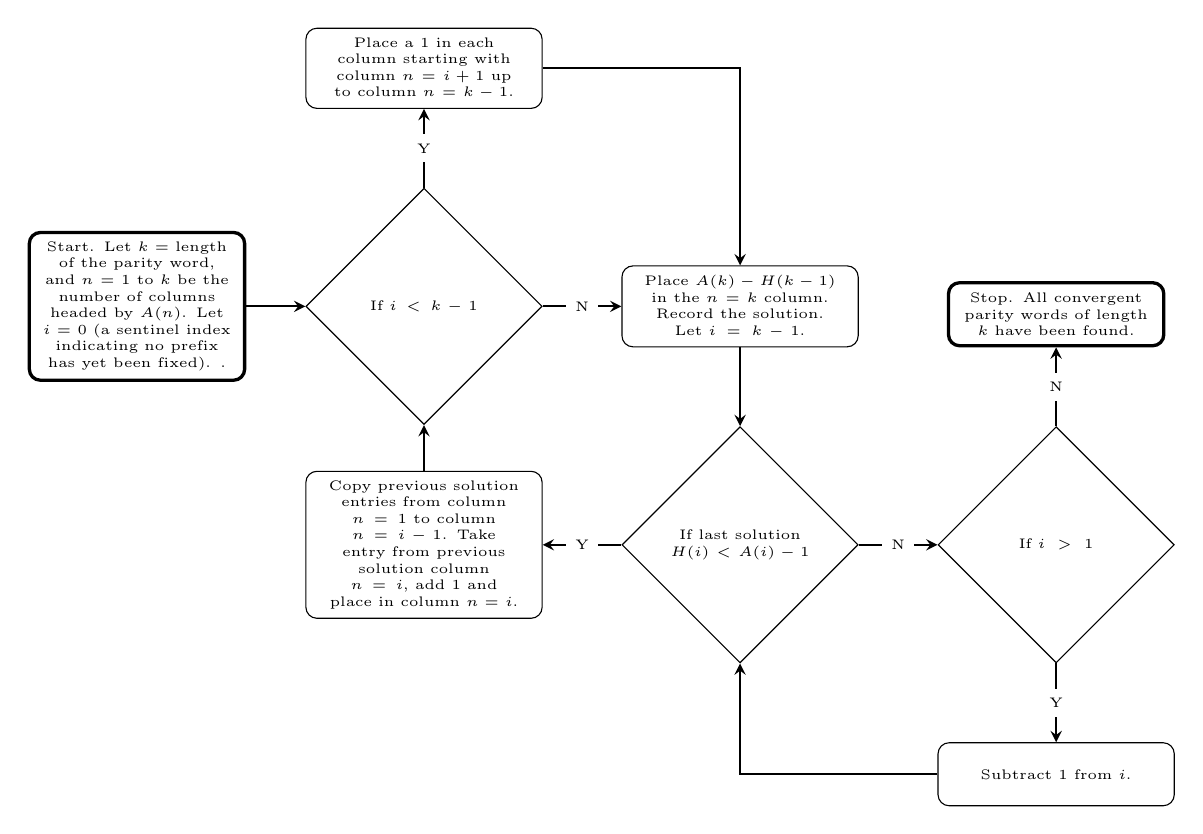
\begin{tikzpicture}[node distance=0.75cm, font = \tiny] % Default node spacing and font size

% Place the nodes on the flowchart
\node(start)        [startstop]                           {Start. Let $k$ = length of the parity word, and $n=1$ to $k$ be the number of columns headed by $A(n)$. Let $i=0$ (a sentinel index indicating no prefix has yet been fixed).
.};
\node(i_lt_k-1)     [decision,  right=of start]           {If $i < k-1$};
\node(carry_ones)   [action,    above=1.0cm of i_lt_k-1]  {Place a 1 in each column starting with column $n=i+1$ up to column $n=k-1$.};
\node(remainder)    [action,    right=1.0cm of i_lt_k-1]  {Place $A(k)-H(k-1)$ in the $n=k$ column. Record the solution. Let $i = k-1$. };
\node(i_lt_A)       [decision,  below=1.0cm of remainder] {If last solution $H(i)<A(i)-1$};
\node(copy_inc)     [action,    left=1.0cm of i_lt_A]     {Copy previous solution entries from column $n=1$ to column $n=i-1$. Take entry from previous solution column $n=i$, add 1 and place in column $n=i$.};
\node(i_gt_2)       [decision,  right=1.0cm of i_lt_A]    {If $i>1$};
\node(decrement_i)  [action,    below=1.0cm of i_gt_2]    {Subtract 1 from $i$.};
\node(stop)         [startstop, above=1.0cm of i_gt_2]    {Stop. All convergent parity words of length $k$ have been found.};

% Connect the nodes with arrows
\draw [arrow] (start)        --                       (i_lt_k-1);
\draw [arrow] (i_lt_k-1)     -- node[fill=white,] {Y} (carry_ones);
\draw [arrow] (i_lt_k-1)     -- node[fill=white,] {N} (remainder);
\draw [arrow] (carry_ones)   -|                       (remainder);
\draw [arrow] (remainder)    --                       (i_lt_A);
\draw [arrow] (i_lt_A)       -- node[fill=white,] {Y} (copy_inc);
\draw [arrow] (i_lt_A)       -- node[fill=white,] {N} (i_gt_2);
\draw [arrow] (copy_inc)     --                       (i_lt_k-1);
\draw [arrow] (i_gt_2)       -- node[fill=white,] {Y} (decrement_i);
\draw [arrow] (decrement_i)  -|                       (i_lt_A);
\draw [arrow] (i_gt_2)       -- node[fill=white,] {N} (stop);

\end{tikzpicture}
\end{center}
\end{figure}

For example, the parity word $\{1,1,1,4\}$ has length $k=4$. Its prefix sums
are $H(1\!:\!3)=1,2,3 < A020914(1\!:\!3)$, and the final step $d_3=4$ brings
$H(4)=7=A020914(4)$. This illustrates how the prefix-wise unity bound governs
admissibility, while the final step may reach or even exceed the unity threshold
without violating convergence.

The method begins by creating a table with column headings, $A(n) = A020914(n)$, for
parity words of length $k$ (i.e. $n=1,2,\ldots,k$).  To find novel convergent parity
words, the horizontal sum at every point in the row is strictly less than the column
heading which will be a value taken from \OEIS{A020914}.  The exception is the last
column where the horizontal sum needs to sum up to \emph{exactly} the value in that column.

The rules for finding elements of novel parity words, $tuple(i)$, of length $k$:

\begin{enumerate}
\item The horizontal sum at every point in the row before $A020914(k)$, where $k$ is the
      length of the parity word is less than $A020914(i)$ where $1 \le i < k$,
      i.e. $H(i) = \sum_{j=1}^{i} tuple(j) < A020914(i)$.
\item The horizontal sum of all powers of 2 in a row equals $A020914(k)$, where $k$ is the
      length of the parity word, $H(k) = \sum_{i=1}^{k} tuple(i) = A020914(k) = A(k)$.
\item Continue to search for solutions which satisfy the previous rules until all valid
      combinations are found.
\end{enumerate}

Rule 1 filters out shorter stopping time parity words.  By matching the horizontal sum
of the total number of factors of two for the last column, but remaining strictly less for
previous columns, shorter stopping time solutions are suppressed and not double counted.

The following table was derived utilizing the parity word algorithm depicted in
Figure~\ref{fig:parity-flowchart}.  This shows all admissible parity words of
length $k=5$ satisfying the prefix constraints $H(n)<A020914(n)$ for $n<5$
and $H(5)=A020914(5)=8$.

\begin{table}[h]
\centering
\caption{Admissible parity words for $k=5$ with $A020914(n)$ bounds.}
\label{tab:k5-words}
\begin{tabular}{c|ccccc}
% \textbf{Parity} &   &   & $A(n)$ &   &   \\
\textbf{Word} & $A(1)=2$ & $A(2)=4$ & $A(3)=5$ & $A(4)=7$ & $A(5)=8$ \\ \hline
1 & 1 & 1 & 1 & 1 & 4 \\
2 & 1 & 1 & 1 & 2 & 3 \\
3 & 1 & 1 & 1 & 3 & 2 \\
4 & 1 & 1 & 2 & 1 & 3 \\
5 & 1 & 1 & 2 & 2 & 2 \\
6 & 1 & 2 & 1 & 1 & 3 \\
7 & 1 & 2 & 1 & 2 & 2 \\
\end{tabular}
\end{table}

Note that for $k=5$ there are 7 admissible parity words satisfying the
prefix-wise unity which is given by $A186009(5+1)=7$.  $A186009(k+1)$
tracks the cardinality of admissible parity words of length $k$.

Among the seven admissible parity words for $k=5$, the final word (1,2,1,2,2)
is extremal.  Its prefix sums approach the bounds $A020914(n)$ as closely as possible
for $n=1,\dots,k-1$ without violating the strict inequality.  At the final step $n=k$,
the cumulative sum reaches exactly $H(k)=A020914(k)$, potentially exceeding unity.  

Symbolically, this pattern is $s,d,s,d,d$,showing that maximal admissible growth
may interleave expansion and contraction steps while remaining admissible. All other
parity words remain below the unity boundary at one or more prefix stages, even though
they converge.

This example concretely demonstrates the strict invariant property of the prefix-wise
unity bound described in Remark~\ref{rem:prefix-invariant}.


\newpage
\section{Lower bound of A186009 from A047749}
\label{app:A047749-lower-bound}

The sequence \OEIS{A047749} admits a construction analogous to the horizontal-sum
formulation of \OEIS{A186009}, with the key difference that its terminal doubling
rule is governed by \OEIS{A000034}($n-2$) rather than \OEIS{A022921}. In particular,
\OEIS{A047749} forbids consecutive doublings, whereas such consecutive doublings
occur periodically in \OEIS{A186009}. This structural restriction yields a pointwise
lower bound.

As a consequence of this, there are never \emph{consecutive} doubles in \OEIS{A047749},
whereas this occurs in \OEIS{A186009}.  Therefore,
\begin{equation}
\label{A186009_ge_A047749_all_n}
A047749(n) \le A186009(n+1)\quad \text{for all } n \in \setNo
\end{equation}
 
Moreover, for $n \ge 8$ the inequality is strict:
\begin{equation}
\label{A186009_gt_A047749_n_ge_8}
A047749(n) < A186009(n+1), \quad n \ge 8.
\end{equation}

The index shift accounts solely for the differing initial offsets of the two sequences.
Table \ref{A047749} illustrates the divergence implied by the differing doubling rules;
it is not used in the proof of inequalities.

% A047749 construction as per the modified recursive A100982 algorithm
\begin{center}
	\afterpage{
    \begin{longtable}{@{}rrrrrrrrrrr@{}}
        \label{A047749} \\
        \caption{\OEIS{A047749} Horizontal Sum Formulation} \\

        \toprule
        $n$ & $a_1(n)$ & $a_2(n)$ & $a_3(n)$ & $a_4(n)$ & $a_5(n)$ & $a_6(n)$ & $a_7(n)$ & $a_8(n)$ & $a_9(n)$ & $\sum a_i(n)$ \\
        
        % Horizontal sum table
        \midrule
         0 & 1 &    &     &     &      &      &       &        &       &      1 \\
         1 & 1 &    &     &     &      &      &       &        &       &      1 \\
         2 & 1 &    &     &     &      &      &       &        &       &      1 \\
         3 & 1 &  1 &     &     &      &      &       &        &       &      2 \\
         4 & 1 &  2 &     &     &      &      &       &        &       &      3 \\
         5 & 1 &  3 &   3 &     &      &      &       &        &       &      7 \\
         6 & 1 &  4 &   7 &     &      &      &       &        &       &     12 \\
         7 & 1 &  5 &  12 &  12 &      &      &       &        &       &     30 \\
         8 & 1 &  6 &  18 &  30 &      &      &       &        &       &     55 \\
         9 & 1 &  7 &  25 &  55 &   55 &      &       &        &       &    143 \\
        10 & 1 &  8 &  33 &  88 &  143 &      &       &        &       &    273 \\
        11 & 1 &  9 &  42 & 130 &  273 &  273 &       &        &       &    728 \\
        12 & 1 & 10 &  52 & 182 &  455 &  728 &       &        &       &   1428 \\ 
        13 & 1 & 11 &  63 & 245 &  700 & 1428 &  1428 &        &       &   3876 \\
        14 & 1 & 12 &  75 & 320 & 1020 & 2448 &  3876 &        &       &   7752 \\
        15 & 1 & 13 &  88 & 408 & 1428 & 3876 &  7752 &   7752 &       &  21318 \\
        16 & 1 & 14 & 102 & 510 & 1938 & 5814 & 13566 &  21318 &       &  43263 \\
        17 & 1 & 15 & 117 & 627 & 2565 & 8379 & 21945 &  43263 & 43263 & 120175 \\
        
        \bottomrule
    \end{longtable}
    } % afterpage
\end{center}

Note that the indexing for \OEIS{A186009} begins at $n=1$ whereas the indexing for
\OEIS{A047749} begins at $n=0$.  So when the indices for both series are equal then
\OEIS{A047749} actually has one \emph{additional} term.

The two sequences are identical for the first 8 terms.  Afterwards, \OEIS{A186009}
begins to grow faster, and despite having one extra term $A047749(16) < A100982(16)$.
The gap between the two series accelerates with increasing $n$ due to the periodic
\emph{consecutive} doubling effect of \OEIS{A186009}.

Since the sequence \OEIS{A047749} excludes the non-linear pattern irregularities
inherent in \OEIS{A186009}, it can be probed analytically allowing for determinations
to be made as to how this lesser sequence behaves.

The even and odd integer terms of the \OEIS{A047749} sequence can each be separately
described in closed form using the discrete binomial formulae provided below.

\paragraph{Even-indexed terms of \OEIS{A047749}.}
For $n=2m$, $m\in\setNo$,
\[
a(n) = \frac{1}{2m+1}\binom{3m}{m}.
\]

\paragraph{Odd-indexed terms of \OEIS{A047749}.}
For $n=2m+1$, $m\in\setNo$,
\[
a(n) = \frac{1}{2m+1}\binom{3m+1}{m+1}.
\]

Expanding discrete binomial expressions for even and odd members of \OEIS{A047749}
into smooth representations using Gamma functions.

For even positive numbers, where $\Gamma(x)$ is the Gamma function:
\[
a(n) = \frac{1}{2m+1} \binom{3m}{m} = \frac{\Gamma(3m+1)}{\Gamma(2m+2)\Gamma(m+1)}; n = 2m, m \in \setNo
\]

For odd positive numbers, where $\Gamma(x)$ is the Gamma function:
\[
a(n) = \frac{1}{2m+1} \binom{3m+1}{m+1} = \frac{\Gamma(3m+2)}{\Gamma(2m+2)\Gamma(m+2)}; n = 2m+1, m \in \setNo
\]

The first logarithmic derivative of the Gamma function is given by:

\[
\psi(x) = \frac{d}{dx} \ln \Gamma(x).
\]

For even positive numbers ($n=2m$), the first derivative of the logarithm is:
\[
\frac{d}{dm} \ln \left( \frac{\Gamma(3m+1)}{\Gamma(2m+2)\Gamma(m+1)} \right) = 3 \psi(3m+1) - 2\psi(2m+2) - \psi(m+1)
\]

For odd positive numbers ($n=2m+1$), the first derivative of the logarithm is:
\[
\frac{d}{dm} \ln \left( \frac{\Gamma(3m+2)}{\Gamma(2m+2)\Gamma(m+2)} \right) = 3 \psi(3m+2) - 2\psi(2m+2) - \psi(m+2)
\]

The binomial representations inherit initial conditions analogous to those arising in the Collatz formulation.
When you evaluate the infinite limit of both the even and odd functions, the first derivatives of the logarithm
approach the same value:
\[
\lim_{m \to \infty} \lbrace 3 \psi(3m+1) - 2\psi(2m+2) - \psi(m+1) \rbrace = \ln\!\left(\frac{3^3}{2^2 \cdot 1^1}\right) \simeq 1.9095
\]

Likewise:
\[
\lim_{m \to \infty} \lbrace 3 \psi(3m+2) - 2\psi(2m+2) - \psi(m+2) \rbrace = \ln\!\left(\frac{3^3}{2^2 \cdot 1^1}\right) \simeq 1.9095
\]

The limit follows from the asymptotic expansion $\psi(x) = \ln(x)  + O(1/x)$.
Thus the logarithmic growth per two terms converges to \(\ln(27/4)\), implying
\[
\lim_{n \to \infty} \frac{a(n+2)}{a(n)} = \frac{27}{4}.
\]
Consequently, the exponential growth rate per single term is bounded below by
\[
\sqrt{\frac{27}{4}}.
\]

To the author’s knowledge, this is the first explicit derivation of a nontrivial
exponential lower bound on the growth rate of $\OEIS{A186009}$ obtained via comparison
with a closed-form binomial sequence.


\clearpage
\bibliographystyle{unsrtnat}
\bibliography{src/latex/references}

\end{document}  
